\section{Post-Bach research at the University of Minnesota's Department of Mechanical Engineering}
During the COVID-19 pandemic, I was offered the opportunity to research improvements for a COVID-19 rapid diagnostic reader at the University of Minnesota in John Bischof's group. Dr. Bischof's BioHeat and Mass Transfer (BHMT) group specializes in the thermodynamics of colloidal solutions-- the applications of this research being in areas like cryopreservation and point-of-care diagnostics.

% \subsection{Introduction}
\subsection{Thermal Contrast Amplification Diagnostic Test Reader}

%\parindent 
Thermal contrast amplification (TCA) is a technology platform to improve rapid diagnostics, specifically lateral flow assays (LFAs). Previous BHMT researchers developed this device wherein regions of concentrated gold nanosphere deposits are plasmonically resonated by a moving, 532 nm-wavelength laser to emit heat that is picked up by an IR camera as it and the laser move across the test strip, like the still image depicted in Figure \ref{fig: tca}.

\begin{wrapfigure}[14]{rt} {0.4\textwidth}
\vspace{-2.5cm}
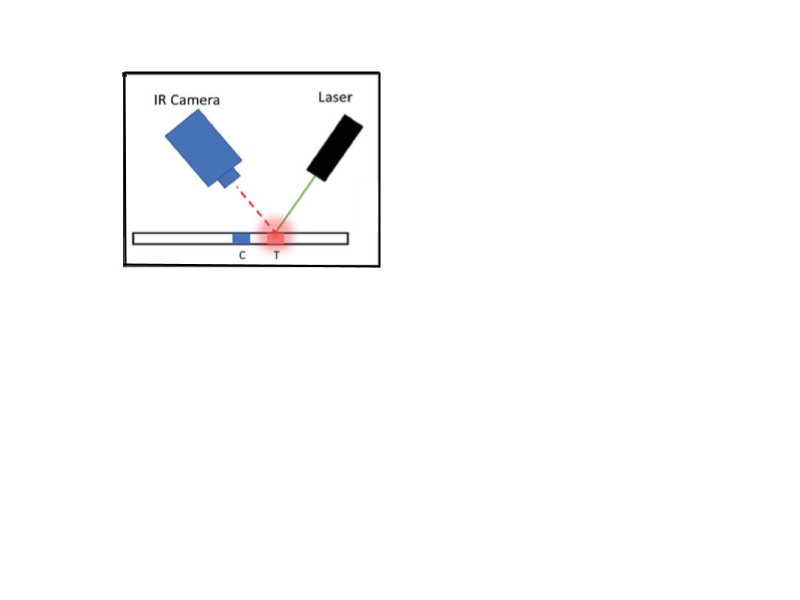
\includegraphics[trim={4cm 0 1cm 0},clip, scale = 0.7]{images/TCA diagram.png}
\vspace{-9cm}
% \parbox{4cm}{
\caption{Schematic for thermal contrast amplification (TCA) focused on the lateral flow assay (LFA) test line (T). Figure snippet from reference \cite{Wang}\label{fig: tca}}
% \vspace{-5cm}
\vfill
\end{wrapfigure}

My initial contributions included making the lateral flow assays being scanned for reading. This process entailed gold nanoparticle (GNP) preparation and synthesis as well as assisting with the specialized dispenser and an automatic cutting paper-cutter. GNP synthesis using the citrate method included characterization with dynamic light scattering (DLS) and spectrophotometry. I would also conjugate antibodies to the GNP I synthesized for use in the testing solution we would run. This testing solution involved buffer selection and optimization to ensure proper antibody binding while minimizing aggregation of the GNPs.

For my third-author publication \cite{Liu} I developed the antibody binding site assay. Briefly, this involved a buffer exchange to set up an off-the-shelf protein crosslinking reaction so I could then use a plate reader to make comparisons between antibody-GNP solutions. My goal was to crosslink antigen and marker molecule with a cleavable bond so that we could assess binding site availability across the industry standard of physical conjugation with our group's covalent conjugation (Figure \ref{fig: rpe-dtt}).
% \newpage
%\\Going through the entire synthesis process: \\
% \noindent
% \hfill{
% \makebox[\textwidth]{
% \restoregeometry

\begin{figure}[ht] 
%{0.4\textwidth}
\vspace{-1cm}
% \hspace{6cm}
\begin{center}
\hspace{2cm}
\justifying{
\adjincludegraphics[trim={0 0 5cm 0}, clip, scale = 0.5]{images/Liu R-PE dtt figures.png}}
\end{center}
\vspace{-10cm}
\caption{Schematic of antigen binding site characterization using PE(phycoerythrin)-antigen conjugate for conjugated gold nanospheres (GNS). Edited figure snippet from reference \cite{Liu}}
%\vspace{-1cm}
\label{fig: rpe-dtt}
\end{figure}

Another consideration of the antibody binding site assay was calculating a molar availability. I was in the process of testing polyacrylamide gel electrophoresis (PAGE) to determine the conjugation ratio of the flourophore-antigen conjugate I synthesized before shifting priorities. The major consideration was that sodium dodecyl sulfate in conventional SDS-PAGE would cleave the disulfide bond in the conjugate, hence I would need to test and select reagents with that in mind.

% \begin{wrapfigure}[17]{r} {0.4\textheight}
\begin{figure}[h]
\centering
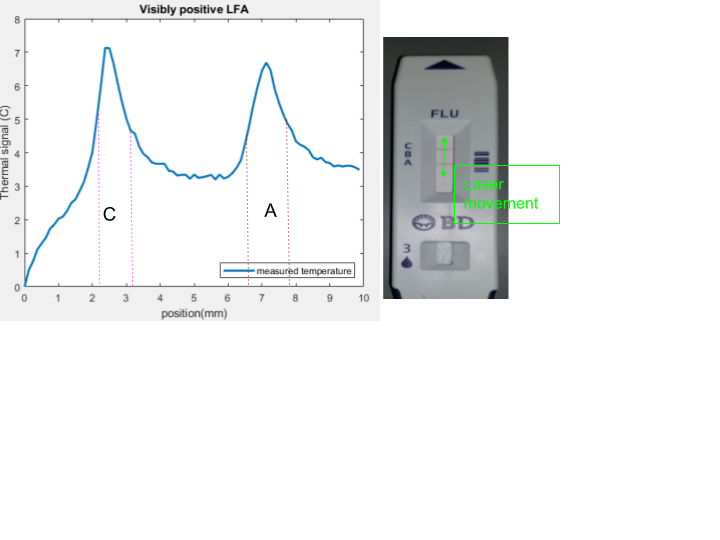
\includegraphics[trim={0 2cm 5cm 0}, clip, scale = 0.5]{images/TCA peaks.png}
\vspace{-2.5cm}
\caption{Side-by-side comparison of thermal readout with laser positioning on the LFA. Thermal signal is a calculation of the IR camera's reading of the laser region subtracted from an established baseline background.}
\label{fig: peaks}
% \vspace{-1cm}
% \end{wrapfigure}
\end{figure}

Computing test determinations following a run was another aspect to the TCA reader. Because regions of high GNP deposition readily heat upon laser exposure, a spike in measured temperature corresponds to antibody binding at the line regions of the LFA (Figure \ref{fig: peaks}). 
%\vspace{-0.5cm}

The specific interests we have in test determination are (a) long stretches of a rise in temperature-- this could correspond to the dispensed line of interest on the LFA and is therefore less likely to be noise-- and (b) large increases-- to indicate the aforementioned deposits of antibody-GNP binding. These interests lead to the selection of a sort of area-under-the-curve (AUC) is used. Where a threshold AUC value for positive tests is determined from a dataset of control tests. The actual calculation is more of an average-under-the-curve where, \begin{center}
\begin{equation} \label{eqn1}
AUC=mean(\Delta T)
\end{equation}
\begin{equation} \label{eqn2}
\Delta T = T(A_{start}:A_{end})-T_{background}
\end{equation}
\end{center} 

With $AUC$ being the average temperature, $\Delta T$, (Equation \ref{eqn1}) across a defined interval of positions $A_{start}:A_{end}$, (Equation \ref{eqn2}) i.e. indices in the $T$ vector, subtracted by a calculated background temperature, $T_{background}$. In the 1.0 version I wrote for the publication \cite{Liu}, I calculated $T_{background}$ from averaging a few points left of $A_{start}$ and a few points right of $A_{end}$. %The chief concern in analyzing a given temperature readout is therefore properly defining $A_{start}:A_{end}$. 
The interval $A_{start}:A_{end}$ represents the test line of the LFA where antibody-GNP binding is expected to occur. This interval is easily estimated by using positive control LFAs to measure out intervals and recording the TCA readout. My 1.0 version was also designed around a generous estimate for human error in physical test placement via a search for the maximum rolling average within a wider interval. These improvements combined with Excel-to-Matlab cross-communication functions I found and added to the code made data processing much more automated, hence a more than 50\% reduction in processing times.

The 2.0 version of the TCA test determination algorithm was designed by the chief technical officer of VigilantDx-- the startup for this test reader. His implementation added a consideration of the control line into the calculations as well as an efficient linear regression for background calculation (Figures \ref{fig: overarching}, \ref{fig: CL}, and \ref{fig: TL}). 

\begin{figure}[h!] 
\begin{center}
%\centering
\subfloat[Summary diagram of test determination algorithm]{
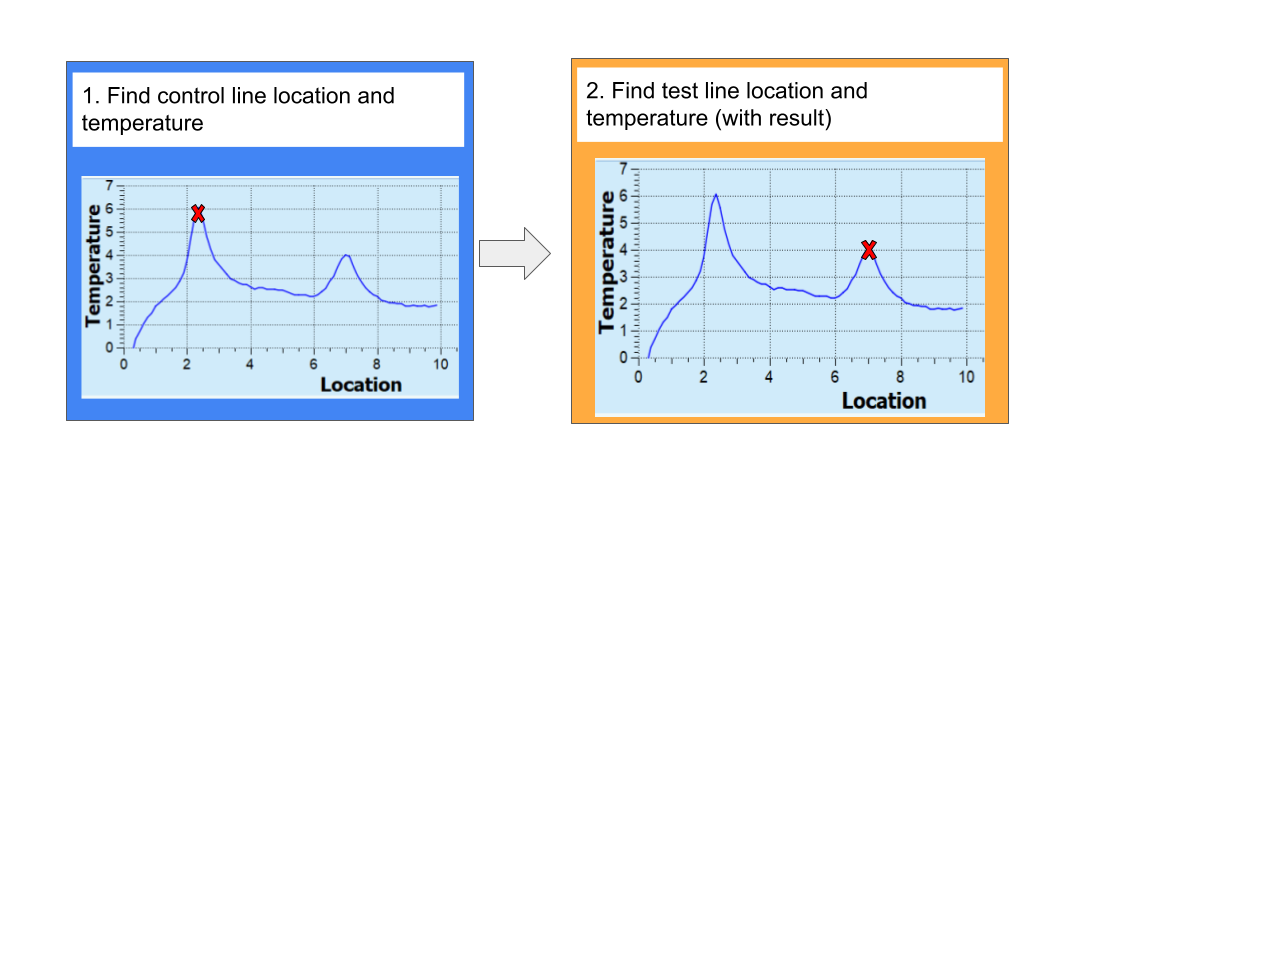
\includegraphics[clip, scale = 0.3]{images/TCA logic a.png}
\vspace{-5.5cm}
\label{fig: overarching}
%\vspace{1.0cm}
}
\end{center}
% \caption{Piecewise flowchart of TCA test determination algorithm version 2.0}
% \label{fig: logic}
% \end{figure}

% \newpage

% \begin{figure}[h!] 
% \ContinuedFloat
\vspace{-1cm}
%\hspace{0.5cm}
%\begin{minipage}[b]{\textwidth}

%\hfill
\begin{center}
\subfloat[Detailed process for control line location]{
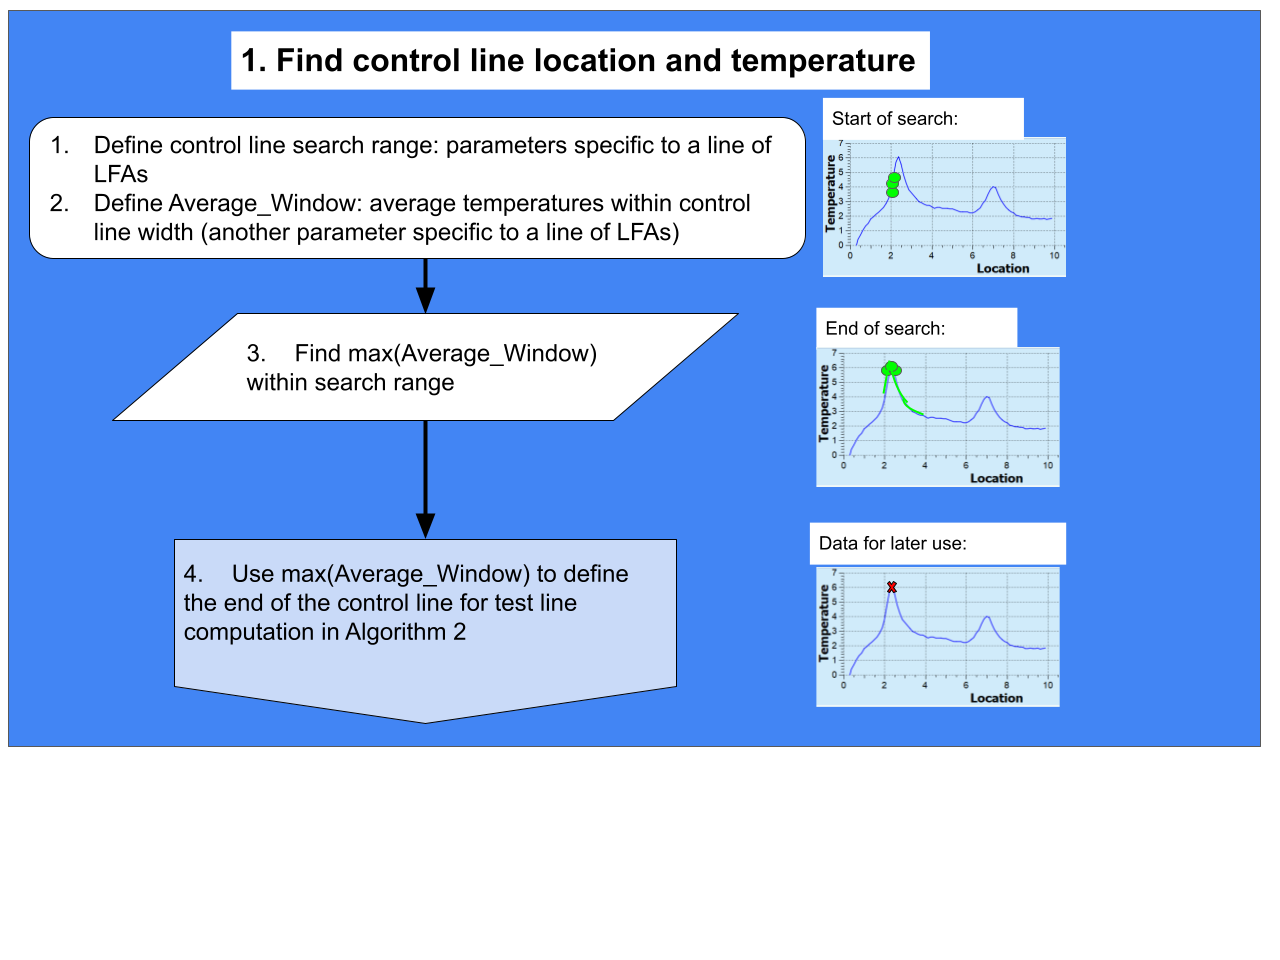
\includegraphics[clip, scale = 0.3]{images/TCA flowchart b.png}
\vspace{-2cm}
\label{fig: CL}
}
%\end{subfigure}
%\hspace{10cm}
\end{center}
\begin{center}
\subfloat[Detailed process for final test determination]{
%\vspace{1cm}
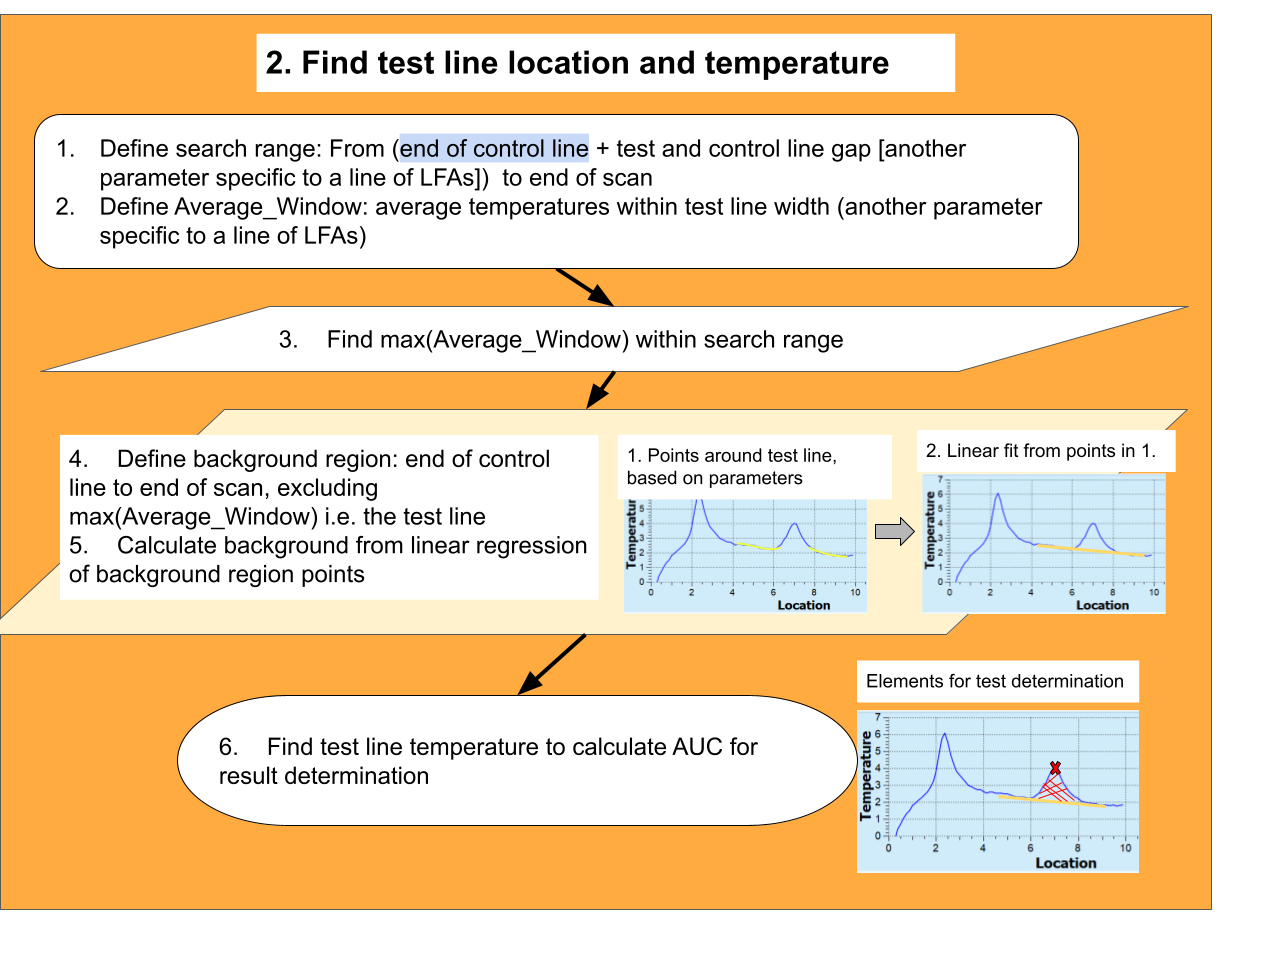
\includegraphics[scale = 0.3]{images/TCA flowchart c.png}
\label{fig: TL}
%\vspace{-1cm}
}
\vspace{-0.5cm}
\end{center}
% \vspace{-1cm}
\caption{Piecewise flowchart of TCA test determination algorithm version 2.0}
\hfill
%\begin{subfigure}[b][3pt][b]{0.2\textwidth}

\hfill
\label{fig: logic1}
\vspace{-1cm}
\end{figure}
%%% If ending here instead of with aquaculture: %%%

% The remainder of my duties involving the TCA reader were validation tests with the 2.0 algorithm and device hardware itself. This project became my primary focus before going on to Carnegie Mellon University for graduate school, I trained my replacement and also wrote and produced instructional manuals and videos for the reader and GNP synthesis.

% \newpage
% \subsection{Aquatic Species Cryopreservation}
% Among the other projects of the BHMT group, I was also involved with the cryopreservation of zebrafish embryos. Building off of previous successes of whole zebrafish embryo cryopreservation in the group \cite{Khosla}, we sought to improve primordial germ cell (PGC) cryopreservation with the procedures used in previous work. PGC cryopreservation allows for a simpler target for vitrification and can easily be transplanted in other fish for efficient husbandry \cite{higaki}-- equivalent to cryopreserving whole embryos if not potentially moreso. \\

% Once I was proficient in microinjection, a key consideration was removing the yolk from the embryo which I had built using parts already available in the research space (Figure \ref{fig: microyolk}). Difficulties in producing a GFP-plasmid for PGC tagging with collaborators kept this project on indeterminate hold and my results with the yolk extractor were purely preliminary before I had to move on. I believe the core parts were adaptable and did not require the exceptional handling required in the previous work's supplemental video \cite{higaki} with fine-tuning primarily for the long-tipped (LT) pipette.
% \newpage
% \vspace{4cm}
% % \begin{figure}[h]
% % \begin{center}
% % \hspace{10cm}
% % \fcapside
% % % \captionsetup[capbesidefigure]
% % %{justification=raggedright}%
% % \thisfloatsetup{capbesideposition=right}
% % % [\FBwidth]
% % % [t]
% % {\caption{Diagram for building a zebrafish yolk extractor from available magnetic microinjection setup.\label{fig: microyolk}}}
% % {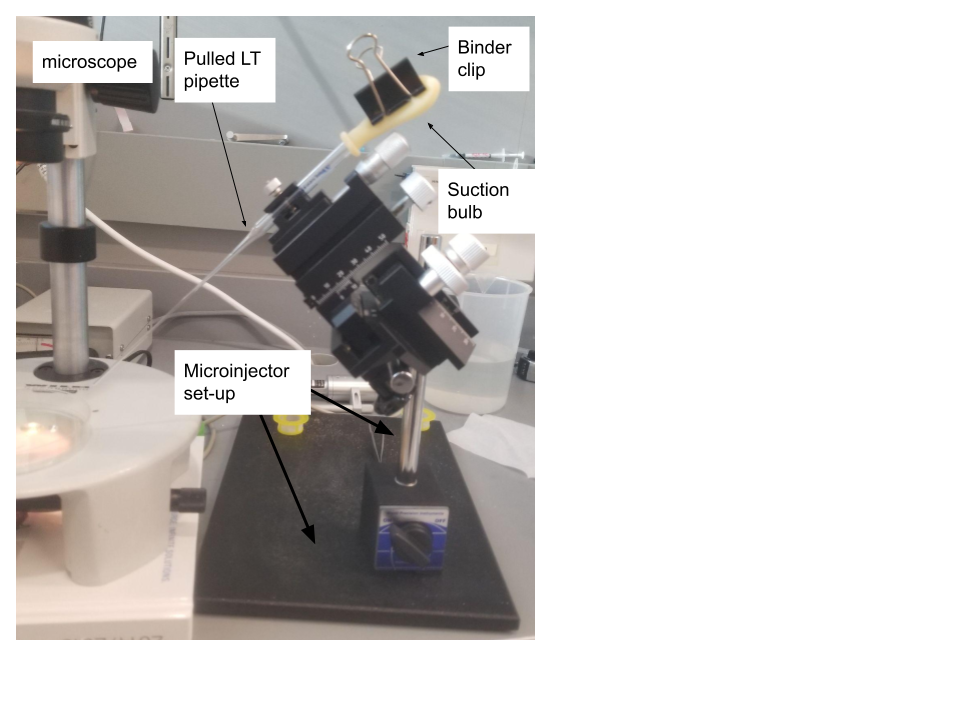
\includegraphics[right, scale = 0.4]{images/Yolk Extraction_embryo digestion.png}}
% % % \end{center}
% % \end{figure}
% % \vspace{4cm}
% \begin{SCfigure}[50][h]
% \vspace{-1cm}
%     % \begin{center}
%     % \justifying{
%     \hspace{2cm}
%     \vspace{5cm}
%     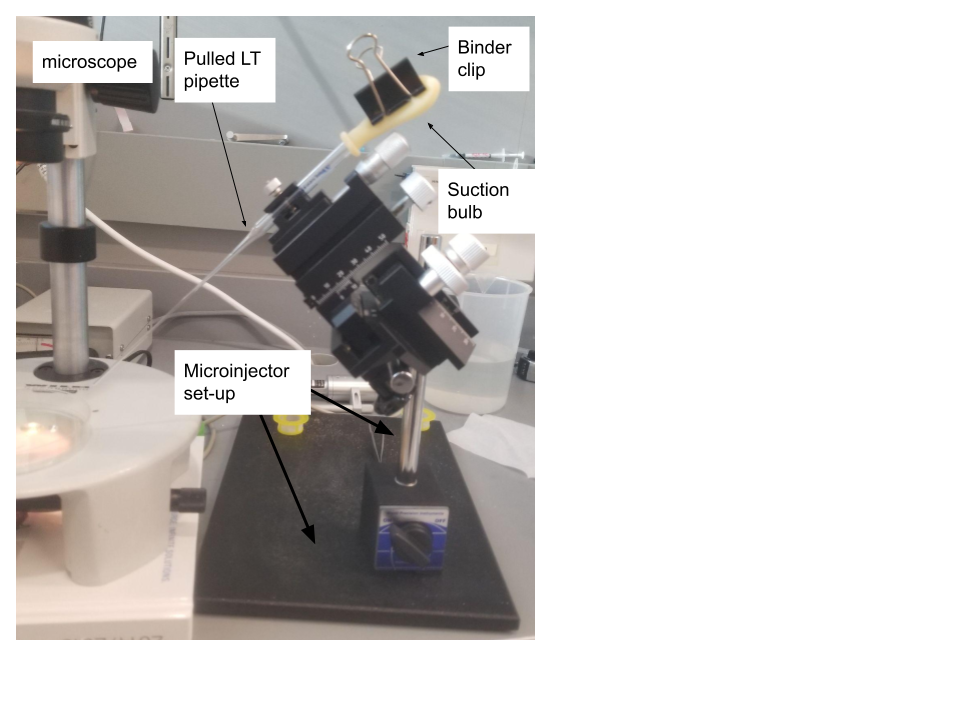
\includegraphics[trim={0 0 15cm 0}, clip, scale = 0.4]{images/Yolk Extraction_embryo digestion.png}    
%         \vspace{-5cm}
%     % \hspace{-8cm}
%     \caption{Diagram for building a zebrafish yolk extractor from available magnetic microinjection setup.}
% \label{fig: microyolk}
%     % \end{center}
%     % \vspace{5cm}
% \end{SCfigure}